\chapter{教学实验和计算实验}
\label{chap:20}

\begin{chapteropening}
观测量、仪器响应和误差预算最终都要回到事件表。桌面 HBT、均匀圆盘拟合、双星可见度、事件表相关器、SPADE 模式排序和 Type Ia 超新星距离 toy model 表面上属于不同题目，输入却都是带时间、通道、偏振和质量标记的光子事件。本章的目标不是罗列几个可以运行的脚本，而是把每个案例都写成一条可检查的观测链：原始事件怎样变成统计量，统计量怎样带入物理模型，模型误差又怎样回到实验设计。HBT 的历史基础、量子光学教学实验、现代强度干涉仪器和模式测量分别见 \citet{1956Natur.178.1046H,1957RSPSA.242..300B,1963PhRv..130.2529G,1963PhRvL..10..277S,1985stop.book.....G,1995ocqo.book.....M,2002SPIE.4588..593L,2024arXiv240418606N,2009A&A...508..531N,2020NatAs...4.1164A,2016PhRvX...6c1033T,2025PhRvD.111h3047K}。
\end{chapteropening}

\section{事件表为什么是一切教学实验的共同语言}

课程的第一步应该让学生看到，事件表不是仪器工程里的琐碎文件格式，而是把光场随机性保留下来的最小记录。平均光变曲线只是事件表的一个投影；一旦先把事件粗分箱，后面就无法重新选择时间窗、通道、偏振、质量筛选或 time-shift 背景。因此实验从事件表开始，事件行采用第 \ref{chap:01} 章式 \eqref{eq:event-row} 的字段，并按第 \ref{chap:06} 章的仪器层要求加入探测器编号、质量标记和时间校正。文件头要写清时间单位是 ns、ps 还是 GPS/UTC 时间戳，探测器编号如何编码，光谱和偏振通道是否存在，质量标记如何记录死时间附近事件、云层、电子学饱和、异常基线或背景窗口。AQuEye、IquEye 和类似光子计数仪器把每个光子保留为时间标签，时间分辨率可到几十 ps，绝对时间通常要用 GPS、铷钟或 White Rabbit 一类同步系统约束到 ns 或亚 ns 量级 \citep{2015SPIE.9504E..0CZ,2016SPIE.9907E..0NZ,2013NIMPA.725..187J,2020RScI...91a3108W}。像 Timepix 这样的像素计数芯片说明，事件表也可以同时带空间位置、能量或到达时间信息 \citep{2007NIMPA.581..485L}。

\begin{figure}[tbp]
\centering
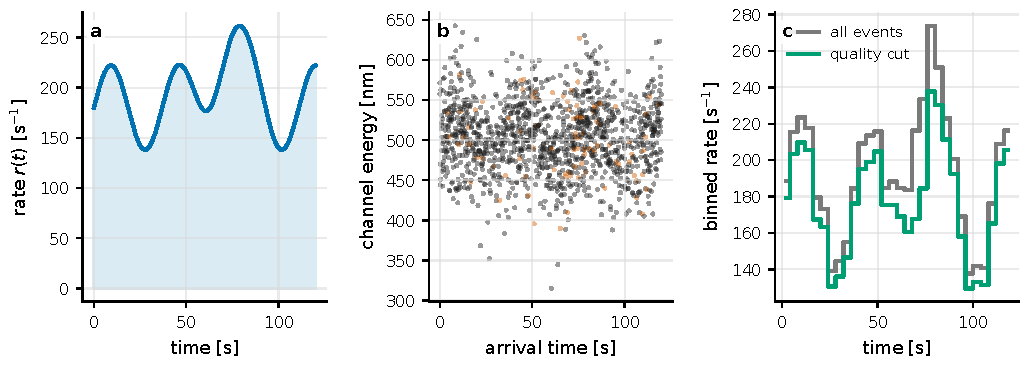
\includegraphics[width=0.96\linewidth]{figures/generated/chapter_20/ch20_event_table_simulation.pdf}
\caption{非齐次 Poisson 过程生成的模拟事件表。左图是输入光子率 \(r(t)\)，中图保留单个光子的到达时间、等效波长通道和质量标记，右图把事件表投影成光变曲线并显示质量筛选的影响。事件表比光变曲线多保留了通道和质量信息，因此同一份数据还能重新用于相关、偏振或能谱分析。}
\label{fig:chapter-20-event-table}
\end{figure}

把事件表投影成光变曲线是一种有损压缩，但它是最容易检查 Poisson 噪声和曝光变化的入口。如果只关心光变曲线，可以把事件表按时间 bin 投影：
\begin{equation}
  n_k = \sum_i {\bf 1}(t_i\in[t_k,t_k+\Delta t))\,{\bf 1}(q_i=1).
  \label{eq:ch20-binned-count}
\end{equation}
\begin{formulaexplain}[公式 (20.1) 解读]
\(n_k\) 是第 \(k\) 个时间 bin 中通过质量筛选的事件数。两个指示函数分别检查到达时间是否落入 bin、事件质量是否合格。
\end{formulaexplain}
\(n_k\) 是第 \(k\) 个 bin 的光子数，没有单位；\(\Delta t\) 是 bin 宽，桌面实验常取 ns 到 ms，天文计时可以从 ns 到分钟；\(q_i=1\) 表示通过质量筛选。估计光子率时 \(r_k=n_k/\Delta t\)，单位是 \({\rm s}^{-1}\)。当每个 bin 内的平均光子数小于几到几十个时，Poisson 噪声不能直接用高斯误差替代；当 \(n_k\gtrsim 30\) 时，高斯近似通常足够。未分箱 Poisson 点过程似然已经在式 \eqref{eq:ch07-point-process-likelihood} 中给出，分箱形式见式 \eqref{eq:ch07-binned-poisson}。同一份事件表既可以直接用事件时间拟合，也可以分箱成光变曲线拟合；两者的比较会显示快速变化和不均匀曝光怎样改变误差。这个形式也能解释为什么 Bayesian Blocks 等事件时间分割方法适合处理脉冲、耀发和强度干涉质量窗口 \citep{2013ApJ...764..167S}。

桌面 HBT 实验要回答的第一个问题是：两路强度各自随机，为什么零延迟附近会比远离零延迟略多一些共同起伏？热光或伪热光可以看成许多相位随机的模式叠加，瞬时强度会涨落；同一个相干时间内分到两个探测器的光子共享这一次强度涨落，所以符合数在 \(\tau=0\) 附近增加。激光直接照到两个探测器时 \(g^{(2)}(0)\simeq1\)，旋转毛玻璃产生的伪热光在单模极限下可以接近 \(g^{(2)}(0)=2\)，多模和有限时间响应会把峰压低 \citep{1991PhRvL..67.1426N,1996PhRvL..76.4344B,1999PhRvA..60..674B,2003PhRvL..91z2301A,2011PhRvL.107u7401C,2024arXiv240418606N}。延迟直方图和 \(g^{(2)}\) 归一化已经在式 \eqref{eq:ch07-pair-count} 和 \eqref{eq:ch07-g2-estimator} 中定义；教学实验要让学生亲手选择 \(\Delta\tau\)、time-shift 背景和质量筛选。若 \(R_1=R_2=5\times10^5\,{\rm s}^{-1}\)、\(T=300\,{\rm s}\)、\(\Delta\tau=0.5\,{\rm ns}\)，随机符合约为 \(3.75\times10^4\) pair/bin，shot-noise 相对误差约 \(1/\sqrt{H}\simeq5\times10^{-3}\)。这个数量级很直观：\(g^{(2)}-1\) 的 \(10^{-2}\) 峰可以在桌面上看见，而 \(10^{-5}\) 的天文聚束峰需要大面积望远镜、长积分和稳定背景。

\begin{figure}[tbp]
\centering
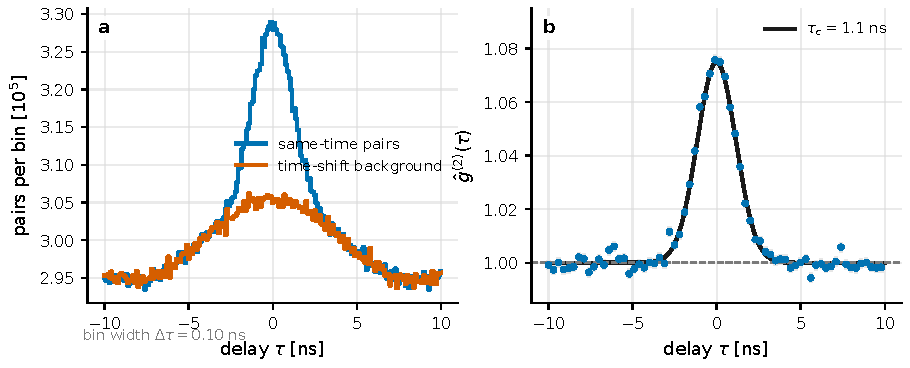
\includegraphics[width=0.96\linewidth]{figures/generated/chapter_20/ch20_hbt_lab_histogram.pdf}
\caption{桌面 HBT 实验的延迟直方图。左图比较同时时间轴的 pair/bin 和 time-shift 背景；慢漂移会同时出现在两条曲线中。右图用背景直方图归一化后得到 \(\hat g^{(2)}(\tau)\)，零延迟附近的峰宽由光源相干时间和探测器响应共同决定。}
\label{fig:chapter-20-hbt}
\end{figure}

真实仪器看到的相关函数是理想 \(g^{(2)}\) 被探测器时间响应卷积后的结果；响应卷积和 jitter budget 见式 \eqref{eq:ch06-response-convolution} 和 \eqref{eq:ch06-jitter-budget}。实验报告应给出响应核的测量方式，而不是只给最终的峰高。若相干时间 \(\tau_c\) 远小于时间 bin 或电子学响应宽度 \(\Delta t\)，热光峰的观测对比度近似按 \(\tau_c/\Delta t\) 稀释。可见光窄带滤光片若中心在 \(416\,{\rm nm}\)、带宽 \(13\,{\rm nm}\)，相干时间只有 \(4\times10^{-14}\,{\rm s}\) 量级；用几 ns 电子学采样时，聚束对比度自然落到 \(10^{-5}\) 量级。学生如果在桌面上只看到一个很漂亮的高峰，反而要追问它来自单模热光、电子串扰、光源慢漂移还是归一化选择。VERITAS、MAGIC 和 Asiago 光子计数实验的强度干涉分析都显式处理这个稀释、背景和死时间问题 \citep{2009A&A...508..531N,2009JMOp...56..261B,2017MNRAS.472.4126G,2020NatAs...4.1164A,2021MNRAS.506.1585Z,2022MNRAS.512.1722K,2024MNRAS.529.4387A,2024ApJ...966...28A}。

\section{桌面 HBT 怎样过渡到恒星角直径和双星}

把 HBT 从桌面搬到两台望远镜后，仍然不是把两处电场直接合束，而是比较两路强度起伏是否同步。区别在于，来自一个有角大小的天体时，两台望远镜接收到的热光涨落不再完全相同；基线越长，两个孔径看到的相干涨落越少，零延迟峰就越低。热光的 Siegert 关系已经在第 \ref{chap:04} 章式 \eqref{eq:ch04-siegert} 中给出，空间强度干涉形式见第 \ref{chap:05} 章式 \eqref{eq:ch05-hbt-spatial} 和 \eqref{eq:ch05-correlation-model}。\(\gamma_{12}\) 表示两台望远镜之间的一阶复相干度，\(|\gamma_{12}|^2\) 等同于天体亮度分布的归一化可见度平方；\(\beta\) 收集时间响应、光谱带宽、偏振选择和仪器效率造成的对比度稀释。若只用单个线偏振、\(\tau_c/\Delta t=10^{-5}\)，则 \(\beta\) 常在 \(10^{-6}\)--\(10^{-5}\) 量级。教学模拟可以故意取 \(\beta=0.05\) 让信号可见，但实验报告要把这个放大因子说清楚。

圆盘星最常用的模型是第 \ref{chap:05} 章式 \eqref{eq:ch05-uniform-disk} 的均匀圆盘，第一零点见式 \eqref{eq:ch05-first-null}。这个案例的教学重点是把每个符号都变成可测量的旋钮：\(\theta\) 是角直径，单位 rad、mas 或 \(\mu{\rm as}\)；\(B_\perp\) 是投影基线，单位 m；\(\lambda\) 是观测波长，单位 m；\(J_1\) 是一阶 Bessel 函数。在 \(\lambda=416\,{\rm nm}\) 时，\(\theta=1\,{\rm mas}\) 的第一零点约在 \(105\,{\rm m}\)。这就是为什么 VERITAS 这类百米级 Cherenkov 阵列可以测亮星角直径，而 Type Ia 超新星的几 \(\mu{\rm as}\) 角半径需要 km 级基线。

\begin{figure}[tbp]
\centering
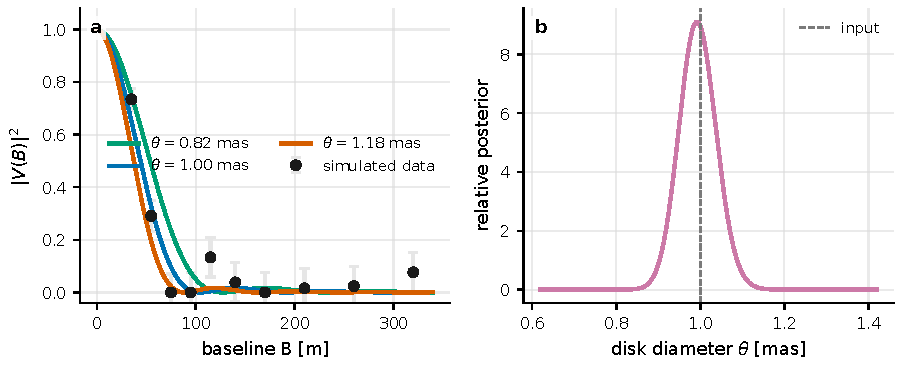
\includegraphics[width=0.96\linewidth]{figures/generated/chapter_20/ch20_uniform_disk_fit.pdf}
\caption{均匀圆盘强度干涉拟合。左图模拟 \(\lambda=416\,{\rm nm}\)、\(\theta=1\,{\rm mas}\) 目标在不同基线上的 \(|V|^2\) 测量；第一零点附近的斜率最大，对角直径最敏感。右图把这些数据转成角直径后验，后验宽度由 \(|V|^2\) 误差、基线覆盖和模型假设共同决定。}
\label{fig:chapter-20-uniform-disk}
\end{figure}

从数据估计 \(|V|^2\) 时，每条基线 \(b\) 先给出零延迟过量相关
\(\hat c_b=\hat g^{(2)}_b(0)-1\)。同夜标定星或实验室标定给出仪器对比度 \(\beta_b\)，于是
\begin{equation}
  \widehat{|V_b|^2}=\frac{\hat c_b}{\hat\beta_b}.
  \label{eq:ch20-v2-estimator}
\end{equation}
\begin{formulaexplain}[公式 (20.2) 解读]
\(\hat c_b\) 是基线 \(b\) 的零延迟相关超额，\(\hat\beta_b\) 是仪器对比度。两者相除才得到天体的 \(|V_b|^2\)，所以校准误差会被直接放大。
\end{formulaexplain}
\(\hat c_b\) 和 \(\hat\beta_b\) 都是无量纲量。若随机符合数为 \(H_b\)，且系统误差暂时忽略，\(\sigma_{\hat c}\simeq H_b^{-1/2}\)。\(\beta\) 一旦小到 \(10^{-5}\)，同样的 \(\sigma_{\hat c}\) 会被放大成 \(\sigma_{|V|^2}\simeq \sigma_{\hat c}/\beta\)。教学模拟若把 \(\beta\) 取得过大，会给出过于漂亮的 \(g^{(2)}\) 峰；天文 \(|V|^2\) 精度仍由真实对比度、随机符合数和系统地板决定。

双星模型让学生看到相位虽然在强度干涉中丢掉了符号，但空间频率振荡仍然保留下来。两点源的 \(|V|^2\) 形式在第 \ref{chap:10} 章式 \eqref{eq:ch10-binary} 和第 \ref{chap:19} 章式 \eqref{eq:ch19-binary-visibility} 已经写出；案例只需把通量比 \(\rho=F_2/F_1\)、角分离向量 \(\boldsymbol s\) 和投影相位 \(2\pi\boldsymbol B_\perp\cdot\boldsymbol s/\lambda\) 放进模拟。 \(\boldsymbol s\) 用 rad 表示，实际写报告常用 mas；\(\boldsymbol B_\perp\cdot\boldsymbol s/\lambda\) 是无量纲相位。等亮双星 \(\rho=1\) 的振荡可以从 1 降到 0；若伴星只有主星 \(10\%\) 的通量，振荡深度约为 \(0.17\)。在 \(B=180\,{\rm m}\)、\(\lambda=500\,{\rm nm}\) 时，\(0.5\,{\rm mas}\) 分离对应相位约 \(5.5\)，单条基线已经能看到明显振荡。轨道拟合时，\(\boldsymbol s(t)\) 随时间变，固定基线也会扫过不同相位。

\begin{figure}[tbp]
\centering
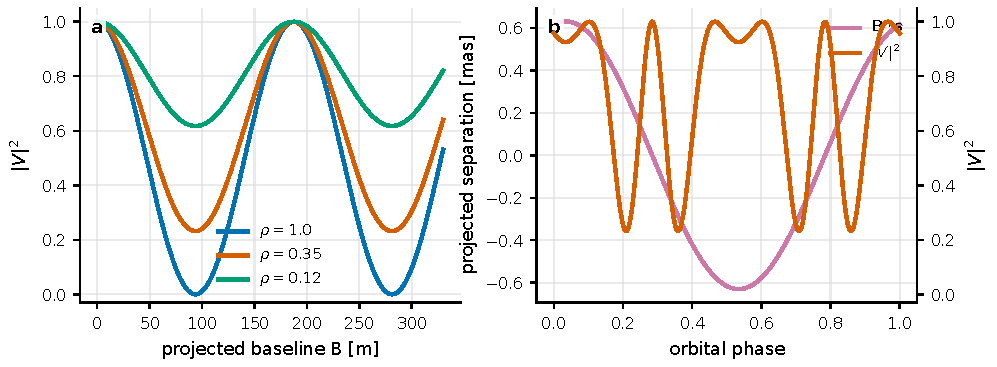
\includegraphics[width=0.96\linewidth]{figures/generated/chapter_20/ch20_binary_visibility.pdf}
\caption{双星 \(|V|^2\) 案例。左图显示固定角分离下通量比 \(\rho\) 如何控制基线振荡深度；右图显示倾斜轨道中投影分离 \(\boldsymbol B\cdot\boldsymbol s\) 随轨道相位变化，并改变固定基线上的 \(|V|^2\)。多基线和多历元数据用来分开分离、通量比和轨道几何。}
\label{fig:chapter-20-binary}
\end{figure}

\section{相关器怎样把事件表变成可检验的相关函数}

相关器案例不要一开始就变成软件性能比赛。先让学生用最朴素的方法确认：相关器的任务是把事件表变成一批延迟直方图或协方差估计；每一个 pair 都必须能追溯到两条原始事件和一个时间差。最朴素的双重循环需要比较所有事件对，计算量随 \(N_1N_2\) 增长；若事件已经按时间排序，只需要比较落在相关窗口 \(|t_j-t_i|<\tau_{\max}\) 内的邻近事件，计算量约为 \(N_\gamma k\)，其中 \(k\sim2R\tau_{\max}\) 是每个事件附近的候选事件数。把事件投影到均匀时间 bin 后，也可以用 FFT 做互相关，计算量约为 \(M\log M\)，\(M=T/\Delta t\)。三种方法估计的是同一个量，但内存、时间 bin 和死时间处理方式不同。

多望远镜阵列的基线数按第 \ref{chap:05} 章式 \eqref{eq:ch05-baseline-number} 随 \(N_{\rm tel}^2\) 增长：4 台望远镜只有 6 条基线，60 台望远镜有 1770 条基线。单望远镜原始数据率的估算见第 \ref{chap:06} 章式 \eqref{eq:ch06-data-rate}；\(\Delta t=4\,{\rm ns}\)、\(N_\nu=1\)、\(n_{\rm bit}=16\) 时，\(D\simeq4\,{\rm Gb\,s^{-1}}\)。若同时保留 64 个光谱通道，单望远镜就到 \(256\,{\rm Gb\,s^{-1}}\)。这解释了为什么现代强度干涉需要 GPU/FPGA 实时相关、分层触发、片上累加或严格的数据压缩；MAGIC 的实时无死时间相关器和 VERITAS 的离线/在线流程都是围绕这个数据率压力设计的 \citep{2020NatAs...4.1164A,2024MNRAS.529.4387A,2024ApJ...966...28A}。

\begin{figure}[tbp]
\centering
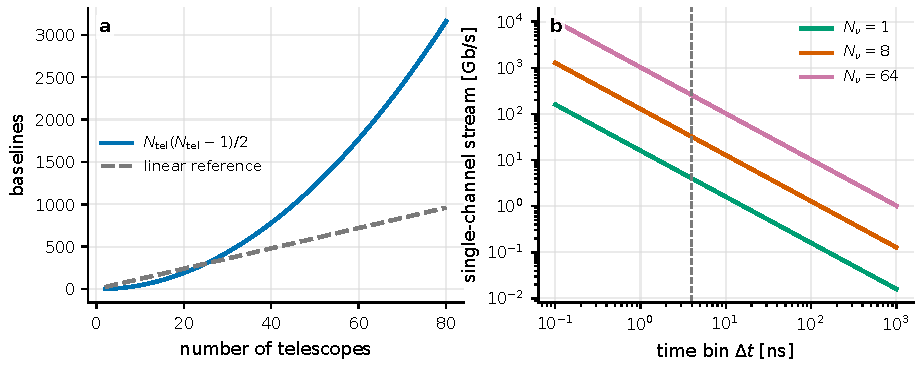
\includegraphics[width=0.96\linewidth]{figures/generated/chapter_20/ch20_correlator_scaling.pdf}
\caption{多望远镜相关器的两个标度。左图显示基线数随望远镜数二次增长，因此阵列扩展会迅速增加相关任务数量。右图显示单路数据流随时间 bin 变窄和光谱通道增多而上升；ns 级采样和几十个光谱通道已经进入需要实时硬件或 GPU 处理的区域。}
\label{fig:chapter-20-correlator}
\end{figure}

相关器案例要包含 null test，而且 null test 应该像结果图一样被评分。把第二路事件整体平移远大于 \(\tau_c\) 的时间后，真实峰应消失；在没有星光或用遮光片时运行同样流程，电子学串扰不应产生零延迟峰；把偏振或光谱通道打乱后，只有物理上应相关的通道保留信号；把数据按时间切片时，\(\hat g^{(2)}(0)-1\) 应随积分时间按 \(T^{-1/2}\) 收敛，而非集中在某一小段。Guerin 等人的实验、AQuEye/IquEye 的光子计数方案以及现代 Cherenkov 阵列强度干涉都说明，这些质量控制直接决定结果能否解释 \citep{2017MNRAS.472.4126G,2016SPIE.9907E..0NZ,2020NatAs...4.1164A,2021MNRAS.506.1585Z,2024MNRAS.529.4387A}。

\section{Rayleigh curse 和 SPADE 教会学生什么}

这一节不是从强度干涉跳到另一个无关主题，而是用一个可计算例子强调同一条思想：仪器记录的默认图像不一定把待估参数的信息放在最显眼的像素里。直接成像用焦平面像素强度估计两点源分离。两个等亮非相干点源的分离 \(s\) 远小于点扩散函数宽度 \(\sigma\) 时，图像几乎只变宽一点点；像素强度对 \(s\) 的导数趋近于零，所以 Fisher 信息下降。这是 Rayleigh curse 在统计上的含义。量子估计理论指出，信息并没有在光场里消失，而是藏在合适的空间模式中 \citep{2015Optic...2..646T,2016PhRvX...6c1033T,2016OExpr..24.3684N,2017PhRvL.118g0801T}。

对高斯点扩散函数和等亮双点源，理想 Hermite--Gaussian 模式排序的概率分布已在第 \ref{chap:08} 章式 \eqref{eq:ch08-spade-probability} 给出。计算实验把 \(n=0,1,2,\ldots\) 当作横向模式编号，并保证分离 \(s\) 和 PSF 宽度 \(\sigma\) 用同一角单位或同一焦平面长度单位。若 \(s=0.2\sigma\)，则控制高阶模式权重的无量纲量为 \(2.5\times10^{-3}\)，绝大多数光子仍在 \(n=0\) 模式，但 \(n=1\) 的小概率变化对 \(s\) 很敏感。理想 SPADE 对分离的 Fisher 信息在 \(s\to0\) 时保持有限；直接像素成像则趋向零。实验上，模式错配、中心定位误差、像差和背景会引入信息地板，所以教学代码应该加入一个可调的模式串扰参数，不宜只画理想曲线。

\begin{figure}[tbp]
\centering
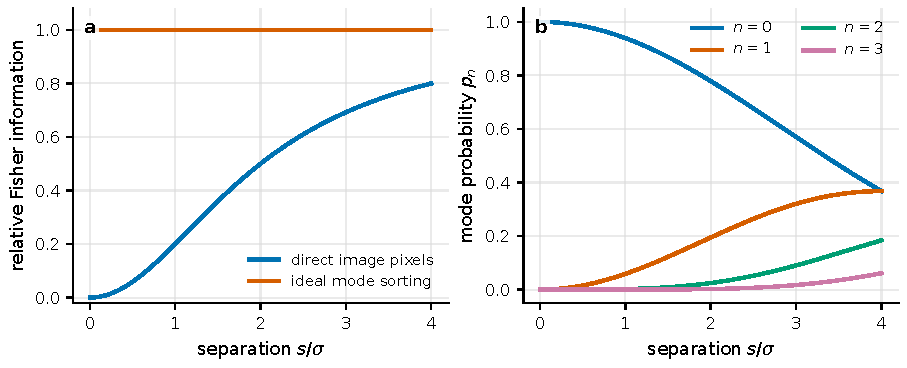
\includegraphics[width=0.96\linewidth]{figures/generated/chapter_20/ch20_spade_computational_experiment.pdf}
\caption{SPADE 计算实验。左图比较小分离处直接像素成像和理想模式排序的相对 Fisher 信息；直接成像在 \(s/\sigma\ll1\) 时信息下降，而模式排序保持接近常数。右图显示 Hermite--Gaussian 模式概率，分离很小时高阶模式概率很小但斜率非零，因此需要高稳定性和低串扰的模式测量。}
\label{fig:chapter-20-spade}
\end{figure}

这个案例和强度干涉指向同一件事：传统图像分辨率不是所有参数的信息极限。强度干涉用 \(|V|^2\) 访问长基线空间频率；SPADE 用模式投影访问直接图像中不显眼的分离信息。实际天文系统会同时面对弱光极限、背景光、多模混合、湍流、像差和探测器效率，因此模式排序更适合作为计算实验和 pathfinder，而不是直接承诺下一代望远镜可以无损达到量子极限。

\section{Type Ia 距离 toy model 怎样串起整套误差预算}

Type Ia 超新星项目把前面几个案例合在一起，也故意暴露最容易被 toy model 掩盖的危险：角半径、速度和爆炸时间看似只差一个比例常数，真实误差却来自不同仪器、不同模型和不同历元。光谱模型给出光球速度 \(v_{\rm ph}(t)\)，强度干涉给出角半径 \(\theta_{\rm ph}(t)\)，二者合成角直径距离：
\begin{equation}
  \theta_{\rm ph}(t)=\frac{R_{\rm ph}(t)}{D_A}
  \simeq \frac{v_{\rm ph}(t-t_0)}{D_A}.
  \label{eq:ch20-typeia-theta}
\end{equation}
\begin{formulaexplain}[公式 (20.3) 解读]
\(\theta_{\rm ph}\) 是光球角半径，\(R_{\rm ph}\) 是物理半径，\(D_A\) 是角直径距离。用速度和时间估计半径，再与角半径比较，就能约束距离。
\end{formulaexplain}
\(v_{\rm ph}\) 的单位是 \({\rm cm\,s^{-1}}\)，正常 Type Ia 在早期常为 \(8\times10^8\)--\(1.5\times10^9\,{\rm cm\,s^{-1}}\)；\(t-t_0\) 的单位是 s 或 d，强度干涉最感兴趣的是爆炸后几天到几十天；\(D_A\) 用 Mpc 表示；\(\theta_{\rm ph}\) 通常是几 \(\mu{\rm as}\) 到几十 \(\mu{\rm as}\)。例如 \(v_{\rm ph}=10^9\,{\rm cm\,s^{-1}}\)、\(t-t_0=15\,{\rm d}\)、\(D_A=20\,{\rm Mpc}\) 时，角半径约 \(4.3\,\mu{\rm as}\)。在 \(\lambda=500\,{\rm nm}\) 下，\(\lambda/\theta\) 对应 \(24\,{\rm km}\) 量级；若利用可见度曲线而不只等第一零点，km 到十 km 级基线仍然有科学信息，但误差预算会非常紧 \citep{2025PhRvD.111h3047K}。

距离后验可以用
\begin{equation}
  \ln{\cal L}(D_A)=
  -\frac{1}{2}\sum_k
  \left[
  \frac{\hat\theta_k-v_{{\rm ph},k}(t_k-t_0)/D_A}
  {\sigma_{\theta,k}}
  \right]^2
  -\frac{1}{2}\sum_k
  \left[
  \frac{\hat v_k-v_{{\rm ph},k}}
  {\sigma_{v,k}}
  \right]^2 .
  \label{eq:ch20-typeia-likelihood}
\end{equation}
\begin{formulaexplain}[公式 (20.4) 解读]
\(D_A\) 是待估距离，\(\hat\theta_k\) 和 \(\hat v_k\) 是第 \(k\) 个历元的角半径与速度观测。似然同时惩罚角半径和速度模型的不一致。
\end{formulaexplain}
\(\hat\theta_k\) 来自第 \(k\) 个历元的 \(|V|^2\) 拟合，单位是 \(\mu{\rm as}\) 或 rad；\(\hat v_k\) 来自光谱线速度或辐射转移模型，单位是 \({\rm cm\,s^{-1}}\)；\(\sigma_{\theta,k}\) 和 \(\sigma_{v,k}\) 分别包括统计误差和模型系统误差。这个 toy model 里若只给 \(\theta\) 加 \(10\%\) 噪声，会得到过于乐观的距离；完整项目还要让学生改变爆炸时间 \(t_0\)、速度梯度、非球对称和亮度分布模型，观察后验怎样变宽。

\begin{figure}[tbp]
\centering
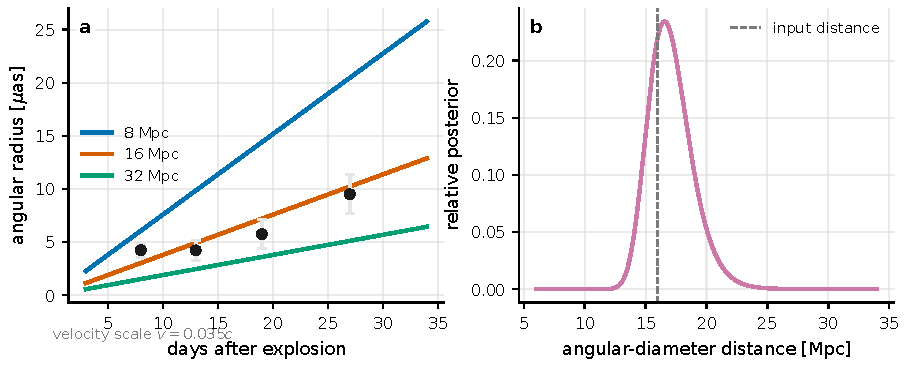
\includegraphics[width=0.96\linewidth]{figures/generated/chapter_20/ch20_typeia_distance_posterior.pdf}
\caption{Type Ia 超新星角直径距离 toy model。左图用 \(v_{\rm ph}=0.035c\) 的简化膨胀模型给出不同距离下的角半径随时间变化，并叠加模拟角半径测量；右图把这些角半径和速度模型合成 \(D_A\) 后验。真实分析需要用辐射转移模型替代常速度球壳，并把非球对称、谱线形成层和基线覆盖写入误差预算。}
\label{fig:chapter-20-typeia}
\end{figure}

课程项目可以按难度递进。最基础的实验用 LED、伪热光和激光测 \(g^{(2)}(\tau)\)，报告 \(R_1,R_2,T,\Delta\tau,\tau_c\) 和响应核 \(K\)。随后用同一份事件表实现 time-shift 背景、质量筛选和 \(T^{-1/2}\) 收敛测试。进入空间相干后，可以拟合均匀圆盘和双星 \(|V|^2\)，比较基线覆盖对 \(\theta\)、\(\rho\) 和 \(\boldsymbol s\) 的影响。更偏信息理论的项目实现 SPADE 概率和 Fisher 信息，并加入模式串扰和中心定位误差。综合项目可以做 Type Ia 距离 toy model，把角半径、速度和爆炸时间的不确定性一起传播。每个项目的产出包括一份事件表说明、一个 Python 脚本、一组 PDF 图、一个引用 ADS bib key 的短报告，以及至少两个 null test。

代码能运行只是第一关。时间相关项目需要说明时间基准、bin 宽、死时间、暗计数和随机符合估计；空间相干项目需要说明 \(B_\perp\)、\(\lambda\)、\(\beta\)、\(|V|^2\) 标定和源模型；模式测量项目需要说明点扩散函数宽度、模式基、串扰矩阵和背景；距离项目需要说明角半径估计、速度模型、爆炸时间和系统误差。缺少这些量时，图仍然可以生成，但结果不能当作天文测量。

